\documentclass[twoside]{book}

% Packages required by doxygen
\usepackage{fixltx2e}
\usepackage{calc}
\usepackage{doxygen}
\usepackage[export]{adjustbox} % also loads graphicx
\usepackage{graphicx}
\usepackage[utf8]{inputenc}
\usepackage{makeidx}
\usepackage{multicol}
\usepackage{multirow}
\PassOptionsToPackage{warn}{textcomp}
\usepackage{textcomp}
\usepackage[nointegrals]{wasysym}
\usepackage[table]{xcolor}

% Font selection
\usepackage[T1]{fontenc}
\usepackage[scaled=.90]{helvet}
\usepackage{courier}
\usepackage{amssymb}
\usepackage{sectsty}
\renewcommand{\familydefault}{\sfdefault}
\allsectionsfont{%
  \fontseries{bc}\selectfont%
  \color{darkgray}%
}
\renewcommand{\DoxyLabelFont}{%
  \fontseries{bc}\selectfont%
  \color{darkgray}%
}
\newcommand{\+}{\discretionary{\mbox{\scriptsize$\hookleftarrow$}}{}{}}

% Page & text layout
\usepackage{geometry}
\geometry{%
  a4paper,%
  top=2.5cm,%
  bottom=2.5cm,%
  left=2.5cm,%
  right=2.5cm%
}
\tolerance=750
\hfuzz=15pt
\hbadness=750
\setlength{\emergencystretch}{15pt}
\setlength{\parindent}{0cm}
\setlength{\parskip}{0.2cm}
\makeatletter
\renewcommand{\paragraph}{%
  \@startsection{paragraph}{4}{0ex}{-1.0ex}{1.0ex}{%
    \normalfont\normalsize\bfseries\SS@parafont%
  }%
}
\renewcommand{\subparagraph}{%
  \@startsection{subparagraph}{5}{0ex}{-1.0ex}{1.0ex}{%
    \normalfont\normalsize\bfseries\SS@subparafont%
  }%
}
\makeatother

% Headers & footers
\usepackage{fancyhdr}
\pagestyle{fancyplain}
\fancyhead[LE]{\fancyplain{}{\bfseries\thepage}}
\fancyhead[CE]{\fancyplain{}{}}
\fancyhead[RE]{\fancyplain{}{\bfseries\leftmark}}
\fancyhead[LO]{\fancyplain{}{\bfseries\rightmark}}
\fancyhead[CO]{\fancyplain{}{}}
\fancyhead[RO]{\fancyplain{}{\bfseries\thepage}}
\fancyfoot[LE]{\fancyplain{}{}}
\fancyfoot[CE]{\fancyplain{}{}}
\fancyfoot[RE]{\fancyplain{}{\bfseries\scriptsize Generated on Wed Oct 7 2015 18\+:02\+:35 for 3\+X\+A3doxy\+Exercise by Doxygen }}
\fancyfoot[LO]{\fancyplain{}{\bfseries\scriptsize Generated on Wed Oct 7 2015 18\+:02\+:35 for 3\+X\+A3doxy\+Exercise by Doxygen }}
\fancyfoot[CO]{\fancyplain{}{}}
\fancyfoot[RO]{\fancyplain{}{}}
\renewcommand{\footrulewidth}{0.4pt}
\renewcommand{\chaptermark}[1]{%
  \markboth{#1}{}%
}
\renewcommand{\sectionmark}[1]{%
  \markright{\thesection\ #1}%
}

% Indices & bibliography
\usepackage{natbib}
\usepackage[titles]{tocloft}
\setcounter{tocdepth}{3}
\setcounter{secnumdepth}{5}
\makeindex

% Hyperlinks (required, but should be loaded last)
\usepackage{ifpdf}
\ifpdf
  \usepackage[pdftex,pagebackref=true]{hyperref}
\else
  \usepackage[ps2pdf,pagebackref=true]{hyperref}
\fi
\hypersetup{%
  colorlinks=true,%
  linkcolor=blue,%
  citecolor=blue,%
  unicode%
}

% Custom commands
\newcommand{\clearemptydoublepage}{%
  \newpage{\pagestyle{empty}\cleardoublepage}%
}


%===== C O N T E N T S =====

\begin{document}

% Titlepage & ToC
\hypersetup{pageanchor=false,
             bookmarks=true,
             bookmarksnumbered=true,
             pdfencoding=unicode
            }
\pagenumbering{roman}
\begin{titlepage}
\vspace*{7cm}
\begin{center}%
{\Large 3\+X\+A3doxy\+Exercise \\[1ex]\large 0.\+1 }\\
\vspace*{1cm}
{\large Generated by Doxygen 1.8.10}\\
\vspace*{0.5cm}
{\small Wed Oct 7 2015 18:02:35}\\
\end{center}
\end{titlepage}
\clearemptydoublepage
\tableofcontents
\clearemptydoublepage
\pagenumbering{arabic}
\hypersetup{pageanchor=true}

%--- Begin generated contents ---
\chapter{Hierarchical Index}
\section{Class Hierarchy}
This inheritance list is sorted roughly, but not completely, alphabetically\+:\begin{DoxyCompactList}
\item Action\+Listener\begin{DoxyCompactList}
\item \contentsline{section}{Menu}{\pageref{class_menu}}{}
\item \contentsline{section}{Options}{\pageref{class_options}}{}
\end{DoxyCompactList}
\item Canvas\begin{DoxyCompactList}
\item \contentsline{section}{Bomberman}{\pageref{class_bomberman}}{}
\end{DoxyCompactList}
\item Item\+Listener\begin{DoxyCompactList}
\item \contentsline{section}{Menu}{\pageref{class_menu}}{}
\item \contentsline{section}{Options}{\pageref{class_options}}{}
\end{DoxyCompactList}
\item J\+Layered\+Pane\begin{DoxyCompactList}
\item \contentsline{section}{Options}{\pageref{class_options}}{}
\end{DoxyCompactList}
\item J\+Menu\+Bar\begin{DoxyCompactList}
\item \contentsline{section}{Menu}{\pageref{class_menu}}{}
\end{DoxyCompactList}
\item Key\+Listener\begin{DoxyCompactList}
\item \contentsline{section}{Bomberman}{\pageref{class_bomberman}}{}
\end{DoxyCompactList}
\item Runnable\begin{DoxyCompactList}
\item \contentsline{section}{Bomb}{\pageref{class_bomb}}{}
\item \contentsline{section}{Player}{\pageref{class_player}}{}
\item \contentsline{section}{Power\+Up}{\pageref{class_power_up}}{}
\item \contentsline{section}{Power\+Up\+Manager}{\pageref{class_power_up_manager}}{}
\end{DoxyCompactList}
\item Change\+Listener\begin{DoxyCompactList}
\item \contentsline{section}{Options}{\pageref{class_options}}{}
\end{DoxyCompactList}
\end{DoxyCompactList}

\chapter{Class Index}
\section{Class List}
Here are the classes, structs, unions and interfaces with brief descriptions\+:\begin{DoxyCompactList}
\item\contentsline{section}{\hyperlink{class_bomb}{Bomb} }{\pageref{class_bomb}}{}
\item\contentsline{section}{\hyperlink{class_bomberman}{Bomberman} }{\pageref{class_bomberman}}{}
\item\contentsline{section}{\hyperlink{class_menu}{Menu} }{\pageref{class_menu}}{}
\item\contentsline{section}{\hyperlink{class_options}{Options} }{\pageref{class_options}}{}
\item\contentsline{section}{\hyperlink{class_player}{Player} }{\pageref{class_player}}{}
\item\contentsline{section}{\hyperlink{class_power_up}{Power\+Up} }{\pageref{class_power_up}}{}
\item\contentsline{section}{\hyperlink{class_power_up_manager}{Power\+Up\+Manager} }{\pageref{class_power_up_manager}}{}
\end{DoxyCompactList}

\chapter{File Index}
\section{File List}
Here is a list of all files with brief descriptions\+:\begin{DoxyCompactList}
\item\contentsline{section}{C\+:/\+Users/\+Ren-\/\+David/workspace/bomber\+Clone/src/\hyperlink{_bomb_8java}{Bomb.\+java} }{\pageref{_bomb_8java}}{}
\item\contentsline{section}{C\+:/\+Users/\+Ren-\/\+David/workspace/bomber\+Clone/src/\hyperlink{_bomberman_8java}{Bomberman.\+java} }{\pageref{_bomberman_8java}}{}
\item\contentsline{section}{C\+:/\+Users/\+Ren-\/\+David/workspace/bomber\+Clone/src/\hyperlink{_menu_8java}{Menu.\+java} }{\pageref{_menu_8java}}{}
\item\contentsline{section}{C\+:/\+Users/\+Ren-\/\+David/workspace/bomber\+Clone/src/\hyperlink{_options_8java}{Options.\+java} }{\pageref{_options_8java}}{}
\item\contentsline{section}{C\+:/\+Users/\+Ren-\/\+David/workspace/bomber\+Clone/src/\hyperlink{_player_8java}{Player.\+java} }{\pageref{_player_8java}}{}
\item\contentsline{section}{C\+:/\+Users/\+Ren-\/\+David/workspace/bomber\+Clone/src/\hyperlink{_power_up_8java}{Power\+Up.\+java} }{\pageref{_power_up_8java}}{}
\item\contentsline{section}{C\+:/\+Users/\+Ren-\/\+David/workspace/bomber\+Clone/src/\hyperlink{_power_up_manager_8java}{Power\+Up\+Manager.\+java} }{\pageref{_power_up_manager_8java}}{}
\end{DoxyCompactList}

\chapter{Class Documentation}
\hypertarget{class_bomb}{}\section{Bomb Class Reference}
\label{class_bomb}\index{Bomb@{Bomb}}
Inheritance diagram for Bomb\+:\begin{figure}[H]
\begin{center}
\leavevmode
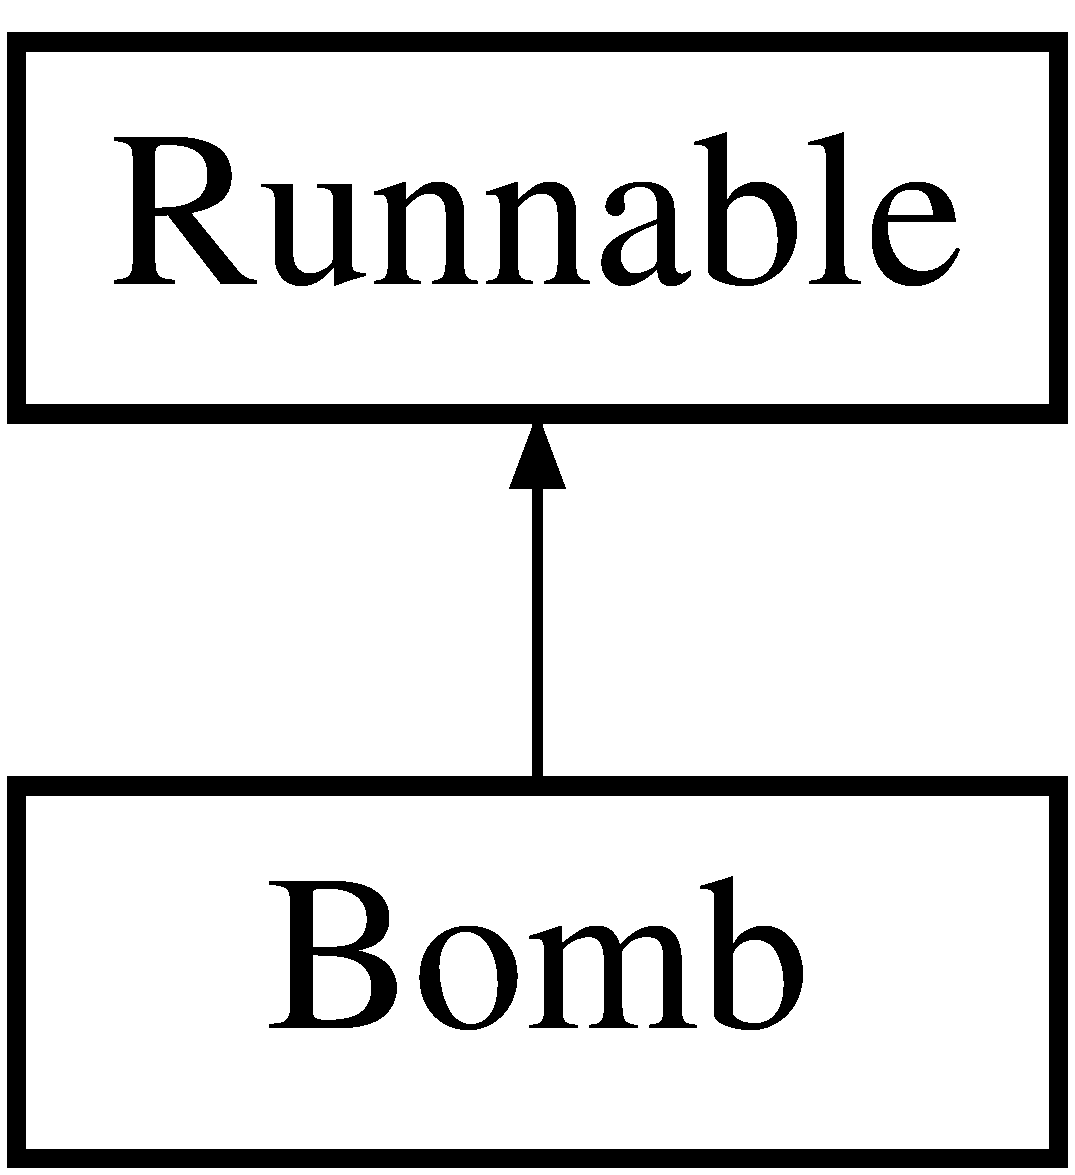
\includegraphics[height=2.000000cm]{class_bomb}
\end{center}
\end{figure}
\subsection*{Public Member Functions}
\begin{DoxyCompactItemize}
\item 
\hyperlink{class_bomb_a33aa40885602ecdae60b1b81fc62651d}{Bomb} (int p, int range)
\item 
\hyperlink{class_bomb_ab721e2d615acb16f662c0bccd8ea8d5f}{Bomb} (int p, int range, int time, int x, int y)
\item 
void \hyperlink{class_bomb_a0e8b8210b1e0d693063e340828a11cfd}{run} ()
\item 
int \hyperlink{class_bomb_a8c56cc0e78d99ac6f323d7c657f9a474}{get\+Grid\+X\+Pos} ()
\item 
int \hyperlink{class_bomb_aaf33f267072aff3b2699a2e2c8010edc}{get\+Grid\+Y\+Pos} ()
\item 
int \hyperlink{class_bomb_a4d7f46b81f4f1828524a22156a1a0541}{get\+Bomb\+Range} ()
\item 
int \hyperlink{class_bomb_a7dfab958f557d250dc9dea7fd4b2cfee}{get\+Player} ()
\item 
void \hyperlink{class_bomb_a5a64459021dc80df15ea52f5873350d7}{detonate\+Bomb} (int x, int y)
\end{DoxyCompactItemize}


\subsection{Constructor \& Destructor Documentation}
\hypertarget{class_bomb_a33aa40885602ecdae60b1b81fc62651d}{}\index{Bomb@{Bomb}!Bomb@{Bomb}}
\index{Bomb@{Bomb}!Bomb@{Bomb}}
\subsubsection[{Bomb(int p, int range)}]{\setlength{\rightskip}{0pt plus 5cm}Bomb.\+Bomb (
\begin{DoxyParamCaption}
\item[{int}]{p, }
\item[{int}]{range}
\end{DoxyParamCaption}
)}\label{class_bomb_a33aa40885602ecdae60b1b81fc62651d}
\hypertarget{class_bomb_ab721e2d615acb16f662c0bccd8ea8d5f}{}\index{Bomb@{Bomb}!Bomb@{Bomb}}
\index{Bomb@{Bomb}!Bomb@{Bomb}}
\subsubsection[{Bomb(int p, int range, int time, int x, int y)}]{\setlength{\rightskip}{0pt plus 5cm}Bomb.\+Bomb (
\begin{DoxyParamCaption}
\item[{int}]{p, }
\item[{int}]{range, }
\item[{int}]{time, }
\item[{int}]{x, }
\item[{int}]{y}
\end{DoxyParamCaption}
)}\label{class_bomb_ab721e2d615acb16f662c0bccd8ea8d5f}


\subsection{Member Function Documentation}
\hypertarget{class_bomb_a5a64459021dc80df15ea52f5873350d7}{}\index{Bomb@{Bomb}!detonate\+Bomb@{detonate\+Bomb}}
\index{detonate\+Bomb@{detonate\+Bomb}!Bomb@{Bomb}}
\subsubsection[{detonate\+Bomb(int x, int y)}]{\setlength{\rightskip}{0pt plus 5cm}void Bomb.\+detonate\+Bomb (
\begin{DoxyParamCaption}
\item[{int}]{x, }
\item[{int}]{y}
\end{DoxyParamCaption}
)}\label{class_bomb_a5a64459021dc80df15ea52f5873350d7}
\hypertarget{class_bomb_a4d7f46b81f4f1828524a22156a1a0541}{}\index{Bomb@{Bomb}!get\+Bomb\+Range@{get\+Bomb\+Range}}
\index{get\+Bomb\+Range@{get\+Bomb\+Range}!Bomb@{Bomb}}
\subsubsection[{get\+Bomb\+Range()}]{\setlength{\rightskip}{0pt plus 5cm}int Bomb.\+get\+Bomb\+Range (
\begin{DoxyParamCaption}
{}
\end{DoxyParamCaption}
)}\label{class_bomb_a4d7f46b81f4f1828524a22156a1a0541}
\hypertarget{class_bomb_a8c56cc0e78d99ac6f323d7c657f9a474}{}\index{Bomb@{Bomb}!get\+Grid\+X\+Pos@{get\+Grid\+X\+Pos}}
\index{get\+Grid\+X\+Pos@{get\+Grid\+X\+Pos}!Bomb@{Bomb}}
\subsubsection[{get\+Grid\+X\+Pos()}]{\setlength{\rightskip}{0pt plus 5cm}int Bomb.\+get\+Grid\+X\+Pos (
\begin{DoxyParamCaption}
{}
\end{DoxyParamCaption}
)}\label{class_bomb_a8c56cc0e78d99ac6f323d7c657f9a474}
\hypertarget{class_bomb_aaf33f267072aff3b2699a2e2c8010edc}{}\index{Bomb@{Bomb}!get\+Grid\+Y\+Pos@{get\+Grid\+Y\+Pos}}
\index{get\+Grid\+Y\+Pos@{get\+Grid\+Y\+Pos}!Bomb@{Bomb}}
\subsubsection[{get\+Grid\+Y\+Pos()}]{\setlength{\rightskip}{0pt plus 5cm}int Bomb.\+get\+Grid\+Y\+Pos (
\begin{DoxyParamCaption}
{}
\end{DoxyParamCaption}
)}\label{class_bomb_aaf33f267072aff3b2699a2e2c8010edc}
\hypertarget{class_bomb_a7dfab958f557d250dc9dea7fd4b2cfee}{}\index{Bomb@{Bomb}!get\+Player@{get\+Player}}
\index{get\+Player@{get\+Player}!Bomb@{Bomb}}
\subsubsection[{get\+Player()}]{\setlength{\rightskip}{0pt plus 5cm}int Bomb.\+get\+Player (
\begin{DoxyParamCaption}
{}
\end{DoxyParamCaption}
)}\label{class_bomb_a7dfab958f557d250dc9dea7fd4b2cfee}
\hypertarget{class_bomb_a0e8b8210b1e0d693063e340828a11cfd}{}\index{Bomb@{Bomb}!run@{run}}
\index{run@{run}!Bomb@{Bomb}}
\subsubsection[{run()}]{\setlength{\rightskip}{0pt plus 5cm}void Bomb.\+run (
\begin{DoxyParamCaption}
{}
\end{DoxyParamCaption}
)}\label{class_bomb_a0e8b8210b1e0d693063e340828a11cfd}


The documentation for this class was generated from the following file\+:\begin{DoxyCompactItemize}
\item 
C\+:/\+Users/\+Ren-\/\+David/workspace/bomber\+Clone/src/\hyperlink{_bomb_8java}{Bomb.\+java}\end{DoxyCompactItemize}

\hypertarget{class_bomberman}{}\section{Bomberman Class Reference}
\label{class_bomberman}\index{Bomberman@{Bomberman}}
Inheritance diagram for Bomberman\+:\begin{figure}[H]
\begin{center}
\leavevmode
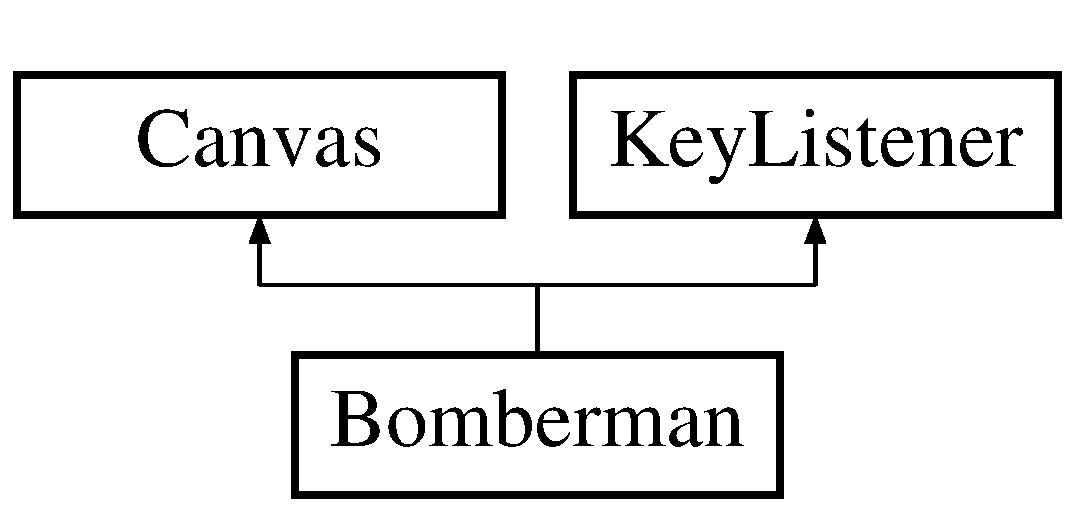
\includegraphics[height=2.000000cm]{class_bomberman}
\end{center}
\end{figure}
\subsection*{Public Member Functions}
\begin{DoxyCompactItemize}
\item 
\hyperlink{class_bomberman_a0390d82a8dbb54267eef4596cb204c1d}{Bomberman} ()
\item 
void \hyperlink{class_bomberman_a29623f557fafadd09713225a2f6e5d87}{game} ()
\item 
void \hyperlink{class_bomberman_aa89f0c27a218cccda9e512a45c1c099e}{key\+Pressed} (Key\+Event event)
\item 
void \hyperlink{class_bomberman_a20612b0e0b2e84367cf8d7f784fab962}{key\+Released} (Key\+Event event)
\item 
void \hyperlink{class_bomberman_a103d91b186f26b2da235de94f0c83f14}{key\+Typed} (Key\+Event event)
\item 
void \hyperlink{class_bomberman_a2987174569eb935f3fb627529eeab3ac}{paint\+Game} ()
\item 
void \hyperlink{class_bomberman_a64949794be90ca1f9c049b107df5eaa0}{update\+Positions} ()
\item 
void \hyperlink{class_bomberman_aba4bf2aeb30f417ba905dee10beedbb9}{check\+Collision} ()
\item 
void \hyperlink{class_bomberman_a3bf6f133b8c0769f51329598ed29b349}{load} ()
\item 
void \hyperlink{class_bomberman_a997783f87885a94d051fcb9a5a849f51}{load\+Map} ()
\item 
void \hyperlink{class_bomberman_a957817254c86d8afe45e7fd2b7c09b24}{check\+Win} ()
\item 
void \hyperlink{class_bomberman_ab0267c9e812ce043cb773db037ccd607}{new\+Game} ()
\item 
void \hyperlink{class_bomberman_ab8373491821d3b4a1cbe41da6b700c64}{create\+Players} ()
\item 
void \hyperlink{class_bomberman_a8bbca3ecf284c927ba263441a49574a4}{options} ()
\item 
void \hyperlink{class_bomberman_a91027bf5033c764e3cf0c445fd8bc0d2}{rules} ()
\item 
void \hyperlink{class_bomberman_aac15074008f535fa531f0182ff5bbe23}{controls} ()
\item 
void \hyperlink{class_bomberman_a050561732a7d0e53daa9980a1dbbcbe7}{credits} ()
\end{DoxyCompactItemize}
\subsection*{Static Public Member Functions}
\begin{DoxyCompactItemize}
\item 
static void \hyperlink{class_bomberman_ab69de0e48af8d28ac2e9bdb58b7074ba}{main} (String\mbox{[}$\,$\mbox{]} args)
\item 
static void \hyperlink{class_bomberman_a54fc0c6fdcd64345d6dedf0afdd7310d}{change\+Sprites} (int n, int p)
\item 
static void \hyperlink{class_bomberman_a1f05f0b836a62ece2b3a05ae50f4c8f7}{initialize} (int players, int bomb\+Limit, int bomb\+Distance, int lives, String map\+Name, String\mbox{[}$\,$\mbox{]} player\+Names)
\end{DoxyCompactItemize}
\subsection*{Public Attributes}
\begin{DoxyCompactItemize}
\item 
Buffer\+Strategy \hyperlink{class_bomberman_a4417f01e97678b10237787d6de283d1c}{bs}
\end{DoxyCompactItemize}
\subsection*{Static Public Attributes}
\begin{DoxyCompactItemize}
\item 
static final int \hyperlink{class_bomberman_a7730b9bf04c6b3bb99edc89e93c13f6c}{W\+I\+D\+T\+H} = 850
\item 
static final int \hyperlink{class_bomberman_acb62777e7ad1e7ba18391ce66ef5b1e2}{H\+E\+I\+G\+H\+T} = 678
\item 
static final int \hyperlink{class_bomberman_a0459d0744420f2371539f445df243505}{S\+P\+E\+E\+D} = 10
\item 
static final int \hyperlink{class_bomberman_ab3f0863e5f567dc7bfc24cd3ef53d8e0}{V\+E\+L\+O\+C\+I\+T\+Y} = 50
\end{DoxyCompactItemize}


\subsection{Detailed Description}
\begin{DoxyAuthor}{Author}
Ren-\/\+David This is the bomberman class 
\end{DoxyAuthor}


\subsection{Constructor \& Destructor Documentation}
\hypertarget{class_bomberman_a0390d82a8dbb54267eef4596cb204c1d}{}\index{Bomberman@{Bomberman}!Bomberman@{Bomberman}}
\index{Bomberman@{Bomberman}!Bomberman@{Bomberman}}
\subsubsection[{Bomberman()}]{\setlength{\rightskip}{0pt plus 5cm}Bomberman.\+Bomberman (
\begin{DoxyParamCaption}
{}
\end{DoxyParamCaption}
)}\label{class_bomberman_a0390d82a8dbb54267eef4596cb204c1d}


\subsection{Member Function Documentation}
\hypertarget{class_bomberman_a54fc0c6fdcd64345d6dedf0afdd7310d}{}\index{Bomberman@{Bomberman}!change\+Sprites@{change\+Sprites}}
\index{change\+Sprites@{change\+Sprites}!Bomberman@{Bomberman}}
\subsubsection[{change\+Sprites(int n, int p)}]{\setlength{\rightskip}{0pt plus 5cm}static void Bomberman.\+change\+Sprites (
\begin{DoxyParamCaption}
\item[{int}]{n, }
\item[{int}]{p}
\end{DoxyParamCaption}
)\hspace{0.3cm}{\ttfamily [static]}}\label{class_bomberman_a54fc0c6fdcd64345d6dedf0afdd7310d}
\hypertarget{class_bomberman_aba4bf2aeb30f417ba905dee10beedbb9}{}\index{Bomberman@{Bomberman}!check\+Collision@{check\+Collision}}
\index{check\+Collision@{check\+Collision}!Bomberman@{Bomberman}}
\subsubsection[{check\+Collision()}]{\setlength{\rightskip}{0pt plus 5cm}void Bomberman.\+check\+Collision (
\begin{DoxyParamCaption}
{}
\end{DoxyParamCaption}
)}\label{class_bomberman_aba4bf2aeb30f417ba905dee10beedbb9}
\hypertarget{class_bomberman_a957817254c86d8afe45e7fd2b7c09b24}{}\index{Bomberman@{Bomberman}!check\+Win@{check\+Win}}
\index{check\+Win@{check\+Win}!Bomberman@{Bomberman}}
\subsubsection[{check\+Win()}]{\setlength{\rightskip}{0pt plus 5cm}void Bomberman.\+check\+Win (
\begin{DoxyParamCaption}
{}
\end{DoxyParamCaption}
)}\label{class_bomberman_a957817254c86d8afe45e7fd2b7c09b24}
\hypertarget{class_bomberman_aac15074008f535fa531f0182ff5bbe23}{}\index{Bomberman@{Bomberman}!controls@{controls}}
\index{controls@{controls}!Bomberman@{Bomberman}}
\subsubsection[{controls()}]{\setlength{\rightskip}{0pt plus 5cm}void Bomberman.\+controls (
\begin{DoxyParamCaption}
{}
\end{DoxyParamCaption}
)}\label{class_bomberman_aac15074008f535fa531f0182ff5bbe23}
\hypertarget{class_bomberman_ab8373491821d3b4a1cbe41da6b700c64}{}\index{Bomberman@{Bomberman}!create\+Players@{create\+Players}}
\index{create\+Players@{create\+Players}!Bomberman@{Bomberman}}
\subsubsection[{create\+Players()}]{\setlength{\rightskip}{0pt plus 5cm}void Bomberman.\+create\+Players (
\begin{DoxyParamCaption}
{}
\end{DoxyParamCaption}
)}\label{class_bomberman_ab8373491821d3b4a1cbe41da6b700c64}
\hypertarget{class_bomberman_a050561732a7d0e53daa9980a1dbbcbe7}{}\index{Bomberman@{Bomberman}!credits@{credits}}
\index{credits@{credits}!Bomberman@{Bomberman}}
\subsubsection[{credits()}]{\setlength{\rightskip}{0pt plus 5cm}void Bomberman.\+credits (
\begin{DoxyParamCaption}
{}
\end{DoxyParamCaption}
)}\label{class_bomberman_a050561732a7d0e53daa9980a1dbbcbe7}
\hypertarget{class_bomberman_a29623f557fafadd09713225a2f6e5d87}{}\index{Bomberman@{Bomberman}!game@{game}}
\index{game@{game}!Bomberman@{Bomberman}}
\subsubsection[{game()}]{\setlength{\rightskip}{0pt plus 5cm}void Bomberman.\+game (
\begin{DoxyParamCaption}
{}
\end{DoxyParamCaption}
)}\label{class_bomberman_a29623f557fafadd09713225a2f6e5d87}
\hypertarget{class_bomberman_a1f05f0b836a62ece2b3a05ae50f4c8f7}{}\index{Bomberman@{Bomberman}!initialize@{initialize}}
\index{initialize@{initialize}!Bomberman@{Bomberman}}
\subsubsection[{initialize(int players, int bomb\+Limit, int bomb\+Distance, int lives, String map\+Name, String[] player\+Names)}]{\setlength{\rightskip}{0pt plus 5cm}static void Bomberman.\+initialize (
\begin{DoxyParamCaption}
\item[{int}]{players, }
\item[{int}]{bomb\+Limit, }
\item[{int}]{bomb\+Distance, }
\item[{int}]{lives, }
\item[{String}]{map\+Name, }
\item[{String\mbox{[}$\,$\mbox{]}}]{player\+Names}
\end{DoxyParamCaption}
)\hspace{0.3cm}{\ttfamily [static]}}\label{class_bomberman_a1f05f0b836a62ece2b3a05ae50f4c8f7}
\hypertarget{class_bomberman_aa89f0c27a218cccda9e512a45c1c099e}{}\index{Bomberman@{Bomberman}!key\+Pressed@{key\+Pressed}}
\index{key\+Pressed@{key\+Pressed}!Bomberman@{Bomberman}}
\subsubsection[{key\+Pressed(\+Key\+Event event)}]{\setlength{\rightskip}{0pt plus 5cm}void Bomberman.\+key\+Pressed (
\begin{DoxyParamCaption}
\item[{Key\+Event}]{event}
\end{DoxyParamCaption}
)}\label{class_bomberman_aa89f0c27a218cccda9e512a45c1c099e}
\hypertarget{class_bomberman_a20612b0e0b2e84367cf8d7f784fab962}{}\index{Bomberman@{Bomberman}!key\+Released@{key\+Released}}
\index{key\+Released@{key\+Released}!Bomberman@{Bomberman}}
\subsubsection[{key\+Released(\+Key\+Event event)}]{\setlength{\rightskip}{0pt plus 5cm}void Bomberman.\+key\+Released (
\begin{DoxyParamCaption}
\item[{Key\+Event}]{event}
\end{DoxyParamCaption}
)}\label{class_bomberman_a20612b0e0b2e84367cf8d7f784fab962}
\hypertarget{class_bomberman_a103d91b186f26b2da235de94f0c83f14}{}\index{Bomberman@{Bomberman}!key\+Typed@{key\+Typed}}
\index{key\+Typed@{key\+Typed}!Bomberman@{Bomberman}}
\subsubsection[{key\+Typed(\+Key\+Event event)}]{\setlength{\rightskip}{0pt plus 5cm}void Bomberman.\+key\+Typed (
\begin{DoxyParamCaption}
\item[{Key\+Event}]{event}
\end{DoxyParamCaption}
)}\label{class_bomberman_a103d91b186f26b2da235de94f0c83f14}
\hypertarget{class_bomberman_a3bf6f133b8c0769f51329598ed29b349}{}\index{Bomberman@{Bomberman}!load@{load}}
\index{load@{load}!Bomberman@{Bomberman}}
\subsubsection[{load()}]{\setlength{\rightskip}{0pt plus 5cm}void Bomberman.\+load (
\begin{DoxyParamCaption}
{}
\end{DoxyParamCaption}
)}\label{class_bomberman_a3bf6f133b8c0769f51329598ed29b349}
\hypertarget{class_bomberman_a997783f87885a94d051fcb9a5a849f51}{}\index{Bomberman@{Bomberman}!load\+Map@{load\+Map}}
\index{load\+Map@{load\+Map}!Bomberman@{Bomberman}}
\subsubsection[{load\+Map()}]{\setlength{\rightskip}{0pt plus 5cm}void Bomberman.\+load\+Map (
\begin{DoxyParamCaption}
{}
\end{DoxyParamCaption}
)}\label{class_bomberman_a997783f87885a94d051fcb9a5a849f51}
\hypertarget{class_bomberman_ab69de0e48af8d28ac2e9bdb58b7074ba}{}\index{Bomberman@{Bomberman}!main@{main}}
\index{main@{main}!Bomberman@{Bomberman}}
\subsubsection[{main(\+String[] args)}]{\setlength{\rightskip}{0pt plus 5cm}static void Bomberman.\+main (
\begin{DoxyParamCaption}
\item[{String\mbox{[}$\,$\mbox{]}}]{args}
\end{DoxyParamCaption}
)\hspace{0.3cm}{\ttfamily [static]}}\label{class_bomberman_ab69de0e48af8d28ac2e9bdb58b7074ba}
\hypertarget{class_bomberman_ab0267c9e812ce043cb773db037ccd607}{}\index{Bomberman@{Bomberman}!new\+Game@{new\+Game}}
\index{new\+Game@{new\+Game}!Bomberman@{Bomberman}}
\subsubsection[{new\+Game()}]{\setlength{\rightskip}{0pt plus 5cm}void Bomberman.\+new\+Game (
\begin{DoxyParamCaption}
{}
\end{DoxyParamCaption}
)}\label{class_bomberman_ab0267c9e812ce043cb773db037ccd607}
\hypertarget{class_bomberman_a8bbca3ecf284c927ba263441a49574a4}{}\index{Bomberman@{Bomberman}!options@{options}}
\index{options@{options}!Bomberman@{Bomberman}}
\subsubsection[{options()}]{\setlength{\rightskip}{0pt plus 5cm}void Bomberman.\+options (
\begin{DoxyParamCaption}
{}
\end{DoxyParamCaption}
)}\label{class_bomberman_a8bbca3ecf284c927ba263441a49574a4}
\hypertarget{class_bomberman_a2987174569eb935f3fb627529eeab3ac}{}\index{Bomberman@{Bomberman}!paint\+Game@{paint\+Game}}
\index{paint\+Game@{paint\+Game}!Bomberman@{Bomberman}}
\subsubsection[{paint\+Game()}]{\setlength{\rightskip}{0pt plus 5cm}void Bomberman.\+paint\+Game (
\begin{DoxyParamCaption}
{}
\end{DoxyParamCaption}
)}\label{class_bomberman_a2987174569eb935f3fb627529eeab3ac}
\hypertarget{class_bomberman_a91027bf5033c764e3cf0c445fd8bc0d2}{}\index{Bomberman@{Bomberman}!rules@{rules}}
\index{rules@{rules}!Bomberman@{Bomberman}}
\subsubsection[{rules()}]{\setlength{\rightskip}{0pt plus 5cm}void Bomberman.\+rules (
\begin{DoxyParamCaption}
{}
\end{DoxyParamCaption}
)}\label{class_bomberman_a91027bf5033c764e3cf0c445fd8bc0d2}
\hypertarget{class_bomberman_a64949794be90ca1f9c049b107df5eaa0}{}\index{Bomberman@{Bomberman}!update\+Positions@{update\+Positions}}
\index{update\+Positions@{update\+Positions}!Bomberman@{Bomberman}}
\subsubsection[{update\+Positions()}]{\setlength{\rightskip}{0pt plus 5cm}void Bomberman.\+update\+Positions (
\begin{DoxyParamCaption}
{}
\end{DoxyParamCaption}
)}\label{class_bomberman_a64949794be90ca1f9c049b107df5eaa0}


\subsection{Member Data Documentation}
\hypertarget{class_bomberman_a4417f01e97678b10237787d6de283d1c}{}\index{Bomberman@{Bomberman}!bs@{bs}}
\index{bs@{bs}!Bomberman@{Bomberman}}
\subsubsection[{bs}]{\setlength{\rightskip}{0pt plus 5cm}Buffer\+Strategy Bomberman.\+bs}\label{class_bomberman_a4417f01e97678b10237787d6de283d1c}
\hypertarget{class_bomberman_acb62777e7ad1e7ba18391ce66ef5b1e2}{}\index{Bomberman@{Bomberman}!H\+E\+I\+G\+H\+T@{H\+E\+I\+G\+H\+T}}
\index{H\+E\+I\+G\+H\+T@{H\+E\+I\+G\+H\+T}!Bomberman@{Bomberman}}
\subsubsection[{H\+E\+I\+G\+H\+T}]{\setlength{\rightskip}{0pt plus 5cm}final int Bomberman.\+H\+E\+I\+G\+H\+T = 678\hspace{0.3cm}{\ttfamily [static]}}\label{class_bomberman_acb62777e7ad1e7ba18391ce66ef5b1e2}
\hypertarget{class_bomberman_a0459d0744420f2371539f445df243505}{}\index{Bomberman@{Bomberman}!S\+P\+E\+E\+D@{S\+P\+E\+E\+D}}
\index{S\+P\+E\+E\+D@{S\+P\+E\+E\+D}!Bomberman@{Bomberman}}
\subsubsection[{S\+P\+E\+E\+D}]{\setlength{\rightskip}{0pt plus 5cm}final int Bomberman.\+S\+P\+E\+E\+D = 10\hspace{0.3cm}{\ttfamily [static]}}\label{class_bomberman_a0459d0744420f2371539f445df243505}
\hypertarget{class_bomberman_ab3f0863e5f567dc7bfc24cd3ef53d8e0}{}\index{Bomberman@{Bomberman}!V\+E\+L\+O\+C\+I\+T\+Y@{V\+E\+L\+O\+C\+I\+T\+Y}}
\index{V\+E\+L\+O\+C\+I\+T\+Y@{V\+E\+L\+O\+C\+I\+T\+Y}!Bomberman@{Bomberman}}
\subsubsection[{V\+E\+L\+O\+C\+I\+T\+Y}]{\setlength{\rightskip}{0pt plus 5cm}final int Bomberman.\+V\+E\+L\+O\+C\+I\+T\+Y = 50\hspace{0.3cm}{\ttfamily [static]}}\label{class_bomberman_ab3f0863e5f567dc7bfc24cd3ef53d8e0}
\hypertarget{class_bomberman_a7730b9bf04c6b3bb99edc89e93c13f6c}{}\index{Bomberman@{Bomberman}!W\+I\+D\+T\+H@{W\+I\+D\+T\+H}}
\index{W\+I\+D\+T\+H@{W\+I\+D\+T\+H}!Bomberman@{Bomberman}}
\subsubsection[{W\+I\+D\+T\+H}]{\setlength{\rightskip}{0pt plus 5cm}final int Bomberman.\+W\+I\+D\+T\+H = 850\hspace{0.3cm}{\ttfamily [static]}}\label{class_bomberman_a7730b9bf04c6b3bb99edc89e93c13f6c}


The documentation for this class was generated from the following file\+:\begin{DoxyCompactItemize}
\item 
C\+:/\+Users/\+Ren-\/\+David/workspace/bomber\+Clone/src/\hyperlink{_bomberman_8java}{Bomberman.\+java}\end{DoxyCompactItemize}

\hypertarget{class_menu}{}\section{Menu Class Reference}
\label{class_menu}\index{Menu@{Menu}}
Inheritance diagram for Menu\+:\begin{figure}[H]
\begin{center}
\leavevmode
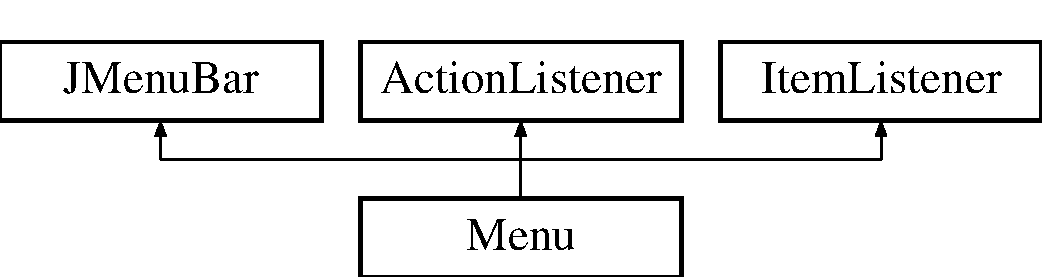
\includegraphics[height=2.000000cm]{class_menu}
\end{center}
\end{figure}
\subsection*{Public Member Functions}
\begin{DoxyCompactItemize}
\item 
\hyperlink{class_menu_a4e07fac071ab4d749fa1d33b959f4b43}{Menu} ()
\item 
void \hyperlink{class_menu_a17ddd90cefc06feb55ec2b1bdc3ae6f9}{action\+Performed} (Action\+Event e)
\item 
void \hyperlink{class_menu_a8dfb067bc4d220470582c5341f3e823d}{item\+State\+Changed} (Item\+Event e)
\end{DoxyCompactItemize}


\subsection{Constructor \& Destructor Documentation}
\hypertarget{class_menu_a4e07fac071ab4d749fa1d33b959f4b43}{}\index{Menu@{Menu}!Menu@{Menu}}
\index{Menu@{Menu}!Menu@{Menu}}
\subsubsection[{Menu()}]{\setlength{\rightskip}{0pt plus 5cm}Menu.\+Menu (
\begin{DoxyParamCaption}
{}
\end{DoxyParamCaption}
)}\label{class_menu_a4e07fac071ab4d749fa1d33b959f4b43}


\subsection{Member Function Documentation}
\hypertarget{class_menu_a17ddd90cefc06feb55ec2b1bdc3ae6f9}{}\index{Menu@{Menu}!action\+Performed@{action\+Performed}}
\index{action\+Performed@{action\+Performed}!Menu@{Menu}}
\subsubsection[{action\+Performed(\+Action\+Event e)}]{\setlength{\rightskip}{0pt plus 5cm}void Menu.\+action\+Performed (
\begin{DoxyParamCaption}
\item[{Action\+Event}]{e}
\end{DoxyParamCaption}
)}\label{class_menu_a17ddd90cefc06feb55ec2b1bdc3ae6f9}
\hypertarget{class_menu_a8dfb067bc4d220470582c5341f3e823d}{}\index{Menu@{Menu}!item\+State\+Changed@{item\+State\+Changed}}
\index{item\+State\+Changed@{item\+State\+Changed}!Menu@{Menu}}
\subsubsection[{item\+State\+Changed(\+Item\+Event e)}]{\setlength{\rightskip}{0pt plus 5cm}void Menu.\+item\+State\+Changed (
\begin{DoxyParamCaption}
\item[{Item\+Event}]{e}
\end{DoxyParamCaption}
)}\label{class_menu_a8dfb067bc4d220470582c5341f3e823d}


The documentation for this class was generated from the following file\+:\begin{DoxyCompactItemize}
\item 
C\+:/\+Users/\+Ren-\/\+David/workspace/bomber\+Clone/src/\hyperlink{_menu_8java}{Menu.\+java}\end{DoxyCompactItemize}

\hypertarget{class_options}{}\section{Options Class Reference}
\label{class_options}\index{Options@{Options}}
Inheritance diagram for Options\+:\begin{figure}[H]
\begin{center}
\leavevmode
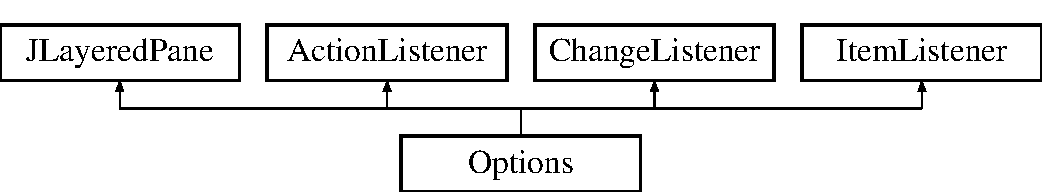
\includegraphics[height=2.000000cm]{class_options}
\end{center}
\end{figure}
\subsection*{Public Member Functions}
\begin{DoxyCompactItemize}
\item 
\hyperlink{class_options_ad09868aa87e39493d69853bdf256e59a}{Options} ()
\item 
void \hyperlink{class_options_a60b78b4fa7ef7d34bab13420794b0b26}{draw\+Map} ()
\item 
void \hyperlink{class_options_a121846a2bdc572b21199167bdcaa8887}{action\+Performed} (Action\+Event e)
\item 
void \hyperlink{class_options_ae985082fcf3bb6df884bd1dd56c72873}{state\+Changed} (Change\+Event e)
\item 
void \hyperlink{class_options_a38bc64ac67fea72d20ce3c95feba60ca}{item\+State\+Changed} (Item\+Event e)
\end{DoxyCompactItemize}


\subsection{Constructor \& Destructor Documentation}
\hypertarget{class_options_ad09868aa87e39493d69853bdf256e59a}{}\index{Options@{Options}!Options@{Options}}
\index{Options@{Options}!Options@{Options}}
\subsubsection[{Options()}]{\setlength{\rightskip}{0pt plus 5cm}Options.\+Options (
\begin{DoxyParamCaption}
{}
\end{DoxyParamCaption}
)}\label{class_options_ad09868aa87e39493d69853bdf256e59a}


\subsection{Member Function Documentation}
\hypertarget{class_options_a121846a2bdc572b21199167bdcaa8887}{}\index{Options@{Options}!action\+Performed@{action\+Performed}}
\index{action\+Performed@{action\+Performed}!Options@{Options}}
\subsubsection[{action\+Performed(\+Action\+Event e)}]{\setlength{\rightskip}{0pt plus 5cm}void Options.\+action\+Performed (
\begin{DoxyParamCaption}
\item[{Action\+Event}]{e}
\end{DoxyParamCaption}
)}\label{class_options_a121846a2bdc572b21199167bdcaa8887}
\hypertarget{class_options_a60b78b4fa7ef7d34bab13420794b0b26}{}\index{Options@{Options}!draw\+Map@{draw\+Map}}
\index{draw\+Map@{draw\+Map}!Options@{Options}}
\subsubsection[{draw\+Map()}]{\setlength{\rightskip}{0pt plus 5cm}void Options.\+draw\+Map (
\begin{DoxyParamCaption}
{}
\end{DoxyParamCaption}
)}\label{class_options_a60b78b4fa7ef7d34bab13420794b0b26}
\hypertarget{class_options_a38bc64ac67fea72d20ce3c95feba60ca}{}\index{Options@{Options}!item\+State\+Changed@{item\+State\+Changed}}
\index{item\+State\+Changed@{item\+State\+Changed}!Options@{Options}}
\subsubsection[{item\+State\+Changed(\+Item\+Event e)}]{\setlength{\rightskip}{0pt plus 5cm}void Options.\+item\+State\+Changed (
\begin{DoxyParamCaption}
\item[{Item\+Event}]{e}
\end{DoxyParamCaption}
)}\label{class_options_a38bc64ac67fea72d20ce3c95feba60ca}
\hypertarget{class_options_ae985082fcf3bb6df884bd1dd56c72873}{}\index{Options@{Options}!state\+Changed@{state\+Changed}}
\index{state\+Changed@{state\+Changed}!Options@{Options}}
\subsubsection[{state\+Changed(\+Change\+Event e)}]{\setlength{\rightskip}{0pt plus 5cm}void Options.\+state\+Changed (
\begin{DoxyParamCaption}
\item[{Change\+Event}]{e}
\end{DoxyParamCaption}
)}\label{class_options_ae985082fcf3bb6df884bd1dd56c72873}


The documentation for this class was generated from the following file\+:\begin{DoxyCompactItemize}
\item 
C\+:/\+Users/\+Ren-\/\+David/workspace/bomber\+Clone/src/\hyperlink{_options_8java}{Options.\+java}\end{DoxyCompactItemize}

\hypertarget{class_player}{}\section{Player Class Reference}
\label{class_player}\index{Player@{Player}}
Inheritance diagram for Player\+:\begin{figure}[H]
\begin{center}
\leavevmode
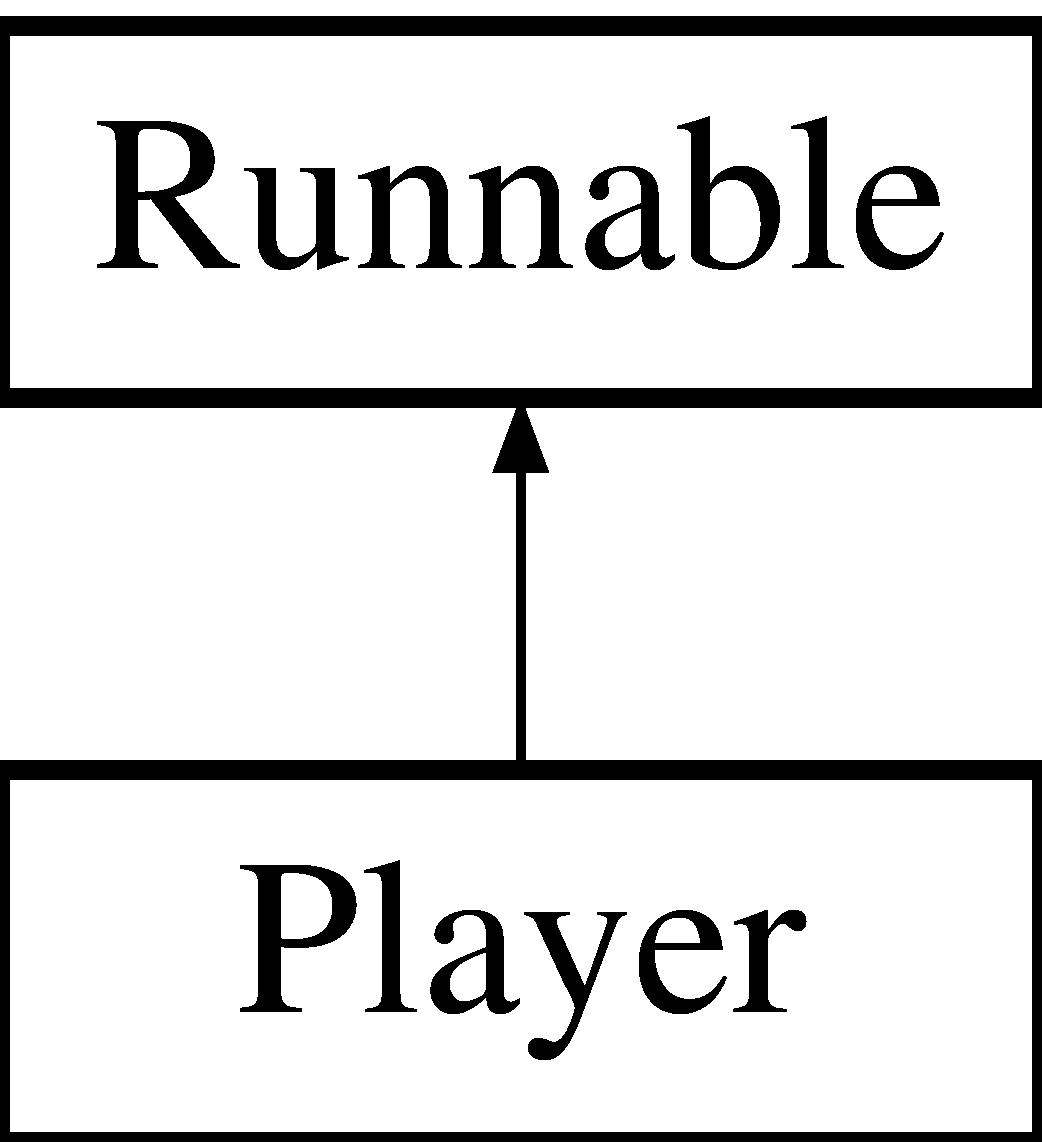
\includegraphics[height=2.000000cm]{class_player}
\end{center}
\end{figure}
\subsection*{Public Member Functions}
\begin{DoxyCompactItemize}
\item 
\hyperlink{class_player_aa276b0ca5f210a31048fb4929e00a6b5}{Player} (int x, int y, int health\+Input, int max\+Bombs\+Input, int range, int p, String n)
\item 
void \hyperlink{class_player_a6169405e26100cc9d10e60d701171d14}{set\+X\+Pos} (int x)
\item 
void \hyperlink{class_player_a20babc9f961a026fcc7aaac5f8769be3}{set\+Y\+Pos} (int y)
\item 
void \hyperlink{class_player_a7ba0f4055816210ab2d9d665552e3a83}{set\+Direction} (int d)
\item 
void \hyperlink{class_player_a8e246afb1a58320ee83182e774ee98fa}{set\+State} (int s)
\item 
void \hyperlink{class_player_a5505703d7d5af25e11a4daceefb03cfe}{increase\+Bomb\+Range} (int r)
\item 
void \hyperlink{class_player_ae2ad118a0435e9414cfa890fe2599784}{increase\+Bomb\+Limit} (int x)
\item 
void \hyperlink{class_player_a3a9cccf5deb51d376068eb572c35a21b}{update\+Health} (int h)
\item 
void \hyperlink{class_player_aa753f19d3b1cc39ec2feaf2311de21bc}{blasted} ()
\item 
void \hyperlink{class_player_a78b1b36f3e4c60cbb278ee4f137d0a47}{bomb\+Used} ()
\item 
void \hyperlink{class_player_a95412f297578bc8cfdf46a538a25e9a2}{phase\+Over} ()
\item 
void \hyperlink{class_player_a30f161013b8d1aab47c651438bafeb30}{bomb\+Exploded} ()
\item 
int \hyperlink{class_player_a458088c2eeff500745b93001ee745bb3}{get\+X\+Pos} ()
\item 
int \hyperlink{class_player_afc249a531c27c856bdda91a93d8ec2e2}{get\+Grid\+X\+Pos} ()
\item 
int \hyperlink{class_player_a382e547f48d5d081e5edec8439d94cff}{get\+Grid\+Y\+Pos} ()
\item 
int \hyperlink{class_player_a49e9b428745bb572aa5380b51b5afb95}{get\+Y\+Pos} ()
\item 
int \hyperlink{class_player_a7ae395cce6cb36c6732e57f31787a381}{get\+Health} ()
\item 
int \hyperlink{class_player_a466088c4480791a464445d96d29877f6}{get\+Direction} ()
\item 
int \hyperlink{class_player_a31698fa7da3e19a859cd2af11c413ecf}{get\+Used\+Bombs} ()
\item 
int \hyperlink{class_player_a7bdbdb3d9b9419225f4a885da14728b5}{get\+Max\+Bombs} ()
\item 
int \hyperlink{class_player_ab11ac70ce6737ab6a7e8ffcda070bdfc}{get\+Bomb\+Range} ()
\item 
int \hyperlink{class_player_a152c1cbd89c6c73639d1e590db2bca9c}{get\+Player\+Num} ()
\item 
int \hyperlink{class_player_ac2518937ade66e10dc5093a6f7bdd8a6}{get\+State} ()
\item 
String \hyperlink{class_player_a7b17595bbe9876d4aa469ad9bee644dd}{get\+Name} ()
\item 
boolean \hyperlink{class_player_a18a27ee5d3e5d698a172391179e672a5}{check\+Post\+Phase} ()
\item 
void \hyperlink{class_player_ad470883cce200d3933fbf5c4ce6465a6}{run} ()
\item 
void \hyperlink{class_player_a3a45889c4b4bc78d219caed03dd04ec7}{reset\+Bomb\+Key} (int p)
\end{DoxyCompactItemize}
\subsection*{Private Attributes}
\begin{DoxyCompactItemize}
\item 
int \hyperlink{class_player_ab064f330cef84e2e062fd6446db24184}{health} = 0
\item 
int \hyperlink{class_player_a280608b62fdcd7f31cb54cf0787cff7f}{x\+Pos} = 0
\item 
int \hyperlink{class_player_aa2706c56cfb101d02b73e371cfb98cd1}{y\+Pos} = 0
\item 
int \hyperlink{class_player_acb502d33ffa4e20bd1d275126dc471ed}{max\+Bombs} = 0
\item 
int \hyperlink{class_player_ab6fd5604046c7ddee01bd5f9b9e69341}{used\+Bombs} = 0
\item 
int \hyperlink{class_player_ae8871f87983cdc59d20c9408b1db88af}{bomb\+Range} = 0
\item 
int \hyperlink{class_player_a497a7481dfd1f564d9cfcc45cc470e1f}{player\+Num} = 0
\item 
boolean \hyperlink{class_player_a961b7def0b24fdb72ded51d4bb15c6d0}{post\+Phase} = false
\item 
int \hyperlink{class_player_a43caa331c7c9f40c51862ad1ebb439ba}{direction} = 0
\item 
Thread \hyperlink{class_player_a2b205a0aba33f0cd4a4b6bbb9b03df35}{timer}
\item 
int \hyperlink{class_player_a73f30624033a23aa5bc290103528e77e}{state} = 0
\item 
boolean \hyperlink{class_player_a8e3ab9f7eed5d3b80be53d3b617d718b}{alive} = true
\item 
String \hyperlink{class_player_aa70e75b3cc209ea82a17c469de0f159c}{name} = \char`\"{}\char`\"{}
\end{DoxyCompactItemize}


\subsection{Constructor \& Destructor Documentation}
\hypertarget{class_player_aa276b0ca5f210a31048fb4929e00a6b5}{}\index{Player@{Player}!Player@{Player}}
\index{Player@{Player}!Player@{Player}}
\subsubsection[{Player(int x, int y, int health\+Input, int max\+Bombs\+Input, int range, int p, String n)}]{\setlength{\rightskip}{0pt plus 5cm}Player.\+Player (
\begin{DoxyParamCaption}
\item[{int}]{x, }
\item[{int}]{y, }
\item[{int}]{health\+Input, }
\item[{int}]{max\+Bombs\+Input, }
\item[{int}]{range, }
\item[{int}]{p, }
\item[{String}]{n}
\end{DoxyParamCaption}
)}\label{class_player_aa276b0ca5f210a31048fb4929e00a6b5}


\subsection{Member Function Documentation}
\hypertarget{class_player_aa753f19d3b1cc39ec2feaf2311de21bc}{}\index{Player@{Player}!blasted@{blasted}}
\index{blasted@{blasted}!Player@{Player}}
\subsubsection[{blasted()}]{\setlength{\rightskip}{0pt plus 5cm}void Player.\+blasted (
\begin{DoxyParamCaption}
{}
\end{DoxyParamCaption}
)}\label{class_player_aa753f19d3b1cc39ec2feaf2311de21bc}
\hypertarget{class_player_a30f161013b8d1aab47c651438bafeb30}{}\index{Player@{Player}!bomb\+Exploded@{bomb\+Exploded}}
\index{bomb\+Exploded@{bomb\+Exploded}!Player@{Player}}
\subsubsection[{bomb\+Exploded()}]{\setlength{\rightskip}{0pt plus 5cm}void Player.\+bomb\+Exploded (
\begin{DoxyParamCaption}
{}
\end{DoxyParamCaption}
)}\label{class_player_a30f161013b8d1aab47c651438bafeb30}
\hypertarget{class_player_a78b1b36f3e4c60cbb278ee4f137d0a47}{}\index{Player@{Player}!bomb\+Used@{bomb\+Used}}
\index{bomb\+Used@{bomb\+Used}!Player@{Player}}
\subsubsection[{bomb\+Used()}]{\setlength{\rightskip}{0pt plus 5cm}void Player.\+bomb\+Used (
\begin{DoxyParamCaption}
{}
\end{DoxyParamCaption}
)}\label{class_player_a78b1b36f3e4c60cbb278ee4f137d0a47}
\hypertarget{class_player_a18a27ee5d3e5d698a172391179e672a5}{}\index{Player@{Player}!check\+Post\+Phase@{check\+Post\+Phase}}
\index{check\+Post\+Phase@{check\+Post\+Phase}!Player@{Player}}
\subsubsection[{check\+Post\+Phase()}]{\setlength{\rightskip}{0pt plus 5cm}boolean Player.\+check\+Post\+Phase (
\begin{DoxyParamCaption}
{}
\end{DoxyParamCaption}
)}\label{class_player_a18a27ee5d3e5d698a172391179e672a5}
\hypertarget{class_player_ab11ac70ce6737ab6a7e8ffcda070bdfc}{}\index{Player@{Player}!get\+Bomb\+Range@{get\+Bomb\+Range}}
\index{get\+Bomb\+Range@{get\+Bomb\+Range}!Player@{Player}}
\subsubsection[{get\+Bomb\+Range()}]{\setlength{\rightskip}{0pt plus 5cm}int Player.\+get\+Bomb\+Range (
\begin{DoxyParamCaption}
{}
\end{DoxyParamCaption}
)}\label{class_player_ab11ac70ce6737ab6a7e8ffcda070bdfc}
\hypertarget{class_player_a466088c4480791a464445d96d29877f6}{}\index{Player@{Player}!get\+Direction@{get\+Direction}}
\index{get\+Direction@{get\+Direction}!Player@{Player}}
\subsubsection[{get\+Direction()}]{\setlength{\rightskip}{0pt plus 5cm}int Player.\+get\+Direction (
\begin{DoxyParamCaption}
{}
\end{DoxyParamCaption}
)}\label{class_player_a466088c4480791a464445d96d29877f6}
\hypertarget{class_player_afc249a531c27c856bdda91a93d8ec2e2}{}\index{Player@{Player}!get\+Grid\+X\+Pos@{get\+Grid\+X\+Pos}}
\index{get\+Grid\+X\+Pos@{get\+Grid\+X\+Pos}!Player@{Player}}
\subsubsection[{get\+Grid\+X\+Pos()}]{\setlength{\rightskip}{0pt plus 5cm}int Player.\+get\+Grid\+X\+Pos (
\begin{DoxyParamCaption}
{}
\end{DoxyParamCaption}
)}\label{class_player_afc249a531c27c856bdda91a93d8ec2e2}
\hypertarget{class_player_a382e547f48d5d081e5edec8439d94cff}{}\index{Player@{Player}!get\+Grid\+Y\+Pos@{get\+Grid\+Y\+Pos}}
\index{get\+Grid\+Y\+Pos@{get\+Grid\+Y\+Pos}!Player@{Player}}
\subsubsection[{get\+Grid\+Y\+Pos()}]{\setlength{\rightskip}{0pt plus 5cm}int Player.\+get\+Grid\+Y\+Pos (
\begin{DoxyParamCaption}
{}
\end{DoxyParamCaption}
)}\label{class_player_a382e547f48d5d081e5edec8439d94cff}
\hypertarget{class_player_a7ae395cce6cb36c6732e57f31787a381}{}\index{Player@{Player}!get\+Health@{get\+Health}}
\index{get\+Health@{get\+Health}!Player@{Player}}
\subsubsection[{get\+Health()}]{\setlength{\rightskip}{0pt plus 5cm}int Player.\+get\+Health (
\begin{DoxyParamCaption}
{}
\end{DoxyParamCaption}
)}\label{class_player_a7ae395cce6cb36c6732e57f31787a381}
\hypertarget{class_player_a7bdbdb3d9b9419225f4a885da14728b5}{}\index{Player@{Player}!get\+Max\+Bombs@{get\+Max\+Bombs}}
\index{get\+Max\+Bombs@{get\+Max\+Bombs}!Player@{Player}}
\subsubsection[{get\+Max\+Bombs()}]{\setlength{\rightskip}{0pt plus 5cm}int Player.\+get\+Max\+Bombs (
\begin{DoxyParamCaption}
{}
\end{DoxyParamCaption}
)}\label{class_player_a7bdbdb3d9b9419225f4a885da14728b5}
\hypertarget{class_player_a7b17595bbe9876d4aa469ad9bee644dd}{}\index{Player@{Player}!get\+Name@{get\+Name}}
\index{get\+Name@{get\+Name}!Player@{Player}}
\subsubsection[{get\+Name()}]{\setlength{\rightskip}{0pt plus 5cm}String Player.\+get\+Name (
\begin{DoxyParamCaption}
{}
\end{DoxyParamCaption}
)}\label{class_player_a7b17595bbe9876d4aa469ad9bee644dd}
\hypertarget{class_player_a152c1cbd89c6c73639d1e590db2bca9c}{}\index{Player@{Player}!get\+Player\+Num@{get\+Player\+Num}}
\index{get\+Player\+Num@{get\+Player\+Num}!Player@{Player}}
\subsubsection[{get\+Player\+Num()}]{\setlength{\rightskip}{0pt plus 5cm}int Player.\+get\+Player\+Num (
\begin{DoxyParamCaption}
{}
\end{DoxyParamCaption}
)}\label{class_player_a152c1cbd89c6c73639d1e590db2bca9c}
\hypertarget{class_player_ac2518937ade66e10dc5093a6f7bdd8a6}{}\index{Player@{Player}!get\+State@{get\+State}}
\index{get\+State@{get\+State}!Player@{Player}}
\subsubsection[{get\+State()}]{\setlength{\rightskip}{0pt plus 5cm}int Player.\+get\+State (
\begin{DoxyParamCaption}
{}
\end{DoxyParamCaption}
)}\label{class_player_ac2518937ade66e10dc5093a6f7bdd8a6}
\hypertarget{class_player_a31698fa7da3e19a859cd2af11c413ecf}{}\index{Player@{Player}!get\+Used\+Bombs@{get\+Used\+Bombs}}
\index{get\+Used\+Bombs@{get\+Used\+Bombs}!Player@{Player}}
\subsubsection[{get\+Used\+Bombs()}]{\setlength{\rightskip}{0pt plus 5cm}int Player.\+get\+Used\+Bombs (
\begin{DoxyParamCaption}
{}
\end{DoxyParamCaption}
)}\label{class_player_a31698fa7da3e19a859cd2af11c413ecf}
\hypertarget{class_player_a458088c2eeff500745b93001ee745bb3}{}\index{Player@{Player}!get\+X\+Pos@{get\+X\+Pos}}
\index{get\+X\+Pos@{get\+X\+Pos}!Player@{Player}}
\subsubsection[{get\+X\+Pos()}]{\setlength{\rightskip}{0pt plus 5cm}int Player.\+get\+X\+Pos (
\begin{DoxyParamCaption}
{}
\end{DoxyParamCaption}
)}\label{class_player_a458088c2eeff500745b93001ee745bb3}
\hypertarget{class_player_a49e9b428745bb572aa5380b51b5afb95}{}\index{Player@{Player}!get\+Y\+Pos@{get\+Y\+Pos}}
\index{get\+Y\+Pos@{get\+Y\+Pos}!Player@{Player}}
\subsubsection[{get\+Y\+Pos()}]{\setlength{\rightskip}{0pt plus 5cm}int Player.\+get\+Y\+Pos (
\begin{DoxyParamCaption}
{}
\end{DoxyParamCaption}
)}\label{class_player_a49e9b428745bb572aa5380b51b5afb95}
\hypertarget{class_player_ae2ad118a0435e9414cfa890fe2599784}{}\index{Player@{Player}!increase\+Bomb\+Limit@{increase\+Bomb\+Limit}}
\index{increase\+Bomb\+Limit@{increase\+Bomb\+Limit}!Player@{Player}}
\subsubsection[{increase\+Bomb\+Limit(int x)}]{\setlength{\rightskip}{0pt plus 5cm}void Player.\+increase\+Bomb\+Limit (
\begin{DoxyParamCaption}
\item[{int}]{x}
\end{DoxyParamCaption}
)}\label{class_player_ae2ad118a0435e9414cfa890fe2599784}
\hypertarget{class_player_a5505703d7d5af25e11a4daceefb03cfe}{}\index{Player@{Player}!increase\+Bomb\+Range@{increase\+Bomb\+Range}}
\index{increase\+Bomb\+Range@{increase\+Bomb\+Range}!Player@{Player}}
\subsubsection[{increase\+Bomb\+Range(int r)}]{\setlength{\rightskip}{0pt plus 5cm}void Player.\+increase\+Bomb\+Range (
\begin{DoxyParamCaption}
\item[{int}]{r}
\end{DoxyParamCaption}
)}\label{class_player_a5505703d7d5af25e11a4daceefb03cfe}
\hypertarget{class_player_a95412f297578bc8cfdf46a538a25e9a2}{}\index{Player@{Player}!phase\+Over@{phase\+Over}}
\index{phase\+Over@{phase\+Over}!Player@{Player}}
\subsubsection[{phase\+Over()}]{\setlength{\rightskip}{0pt plus 5cm}void Player.\+phase\+Over (
\begin{DoxyParamCaption}
{}
\end{DoxyParamCaption}
)}\label{class_player_a95412f297578bc8cfdf46a538a25e9a2}
\hypertarget{class_player_a3a45889c4b4bc78d219caed03dd04ec7}{}\index{Player@{Player}!reset\+Bomb\+Key@{reset\+Bomb\+Key}}
\index{reset\+Bomb\+Key@{reset\+Bomb\+Key}!Player@{Player}}
\subsubsection[{reset\+Bomb\+Key(int p)}]{\setlength{\rightskip}{0pt plus 5cm}void Player.\+reset\+Bomb\+Key (
\begin{DoxyParamCaption}
\item[{int}]{p}
\end{DoxyParamCaption}
)}\label{class_player_a3a45889c4b4bc78d219caed03dd04ec7}
\hypertarget{class_player_ad470883cce200d3933fbf5c4ce6465a6}{}\index{Player@{Player}!run@{run}}
\index{run@{run}!Player@{Player}}
\subsubsection[{run()}]{\setlength{\rightskip}{0pt plus 5cm}void Player.\+run (
\begin{DoxyParamCaption}
{}
\end{DoxyParamCaption}
)}\label{class_player_ad470883cce200d3933fbf5c4ce6465a6}
\hypertarget{class_player_a7ba0f4055816210ab2d9d665552e3a83}{}\index{Player@{Player}!set\+Direction@{set\+Direction}}
\index{set\+Direction@{set\+Direction}!Player@{Player}}
\subsubsection[{set\+Direction(int d)}]{\setlength{\rightskip}{0pt plus 5cm}void Player.\+set\+Direction (
\begin{DoxyParamCaption}
\item[{int}]{d}
\end{DoxyParamCaption}
)}\label{class_player_a7ba0f4055816210ab2d9d665552e3a83}
\hypertarget{class_player_a8e246afb1a58320ee83182e774ee98fa}{}\index{Player@{Player}!set\+State@{set\+State}}
\index{set\+State@{set\+State}!Player@{Player}}
\subsubsection[{set\+State(int s)}]{\setlength{\rightskip}{0pt plus 5cm}void Player.\+set\+State (
\begin{DoxyParamCaption}
\item[{int}]{s}
\end{DoxyParamCaption}
)}\label{class_player_a8e246afb1a58320ee83182e774ee98fa}
\hypertarget{class_player_a6169405e26100cc9d10e60d701171d14}{}\index{Player@{Player}!set\+X\+Pos@{set\+X\+Pos}}
\index{set\+X\+Pos@{set\+X\+Pos}!Player@{Player}}
\subsubsection[{set\+X\+Pos(int x)}]{\setlength{\rightskip}{0pt plus 5cm}void Player.\+set\+X\+Pos (
\begin{DoxyParamCaption}
\item[{int}]{x}
\end{DoxyParamCaption}
)}\label{class_player_a6169405e26100cc9d10e60d701171d14}
\hypertarget{class_player_a20babc9f961a026fcc7aaac5f8769be3}{}\index{Player@{Player}!set\+Y\+Pos@{set\+Y\+Pos}}
\index{set\+Y\+Pos@{set\+Y\+Pos}!Player@{Player}}
\subsubsection[{set\+Y\+Pos(int y)}]{\setlength{\rightskip}{0pt plus 5cm}void Player.\+set\+Y\+Pos (
\begin{DoxyParamCaption}
\item[{int}]{y}
\end{DoxyParamCaption}
)}\label{class_player_a20babc9f961a026fcc7aaac5f8769be3}
\hypertarget{class_player_a3a9cccf5deb51d376068eb572c35a21b}{}\index{Player@{Player}!update\+Health@{update\+Health}}
\index{update\+Health@{update\+Health}!Player@{Player}}
\subsubsection[{update\+Health(int h)}]{\setlength{\rightskip}{0pt plus 5cm}void Player.\+update\+Health (
\begin{DoxyParamCaption}
\item[{int}]{h}
\end{DoxyParamCaption}
)}\label{class_player_a3a9cccf5deb51d376068eb572c35a21b}


\subsection{Member Data Documentation}
\hypertarget{class_player_a8e3ab9f7eed5d3b80be53d3b617d718b}{}\index{Player@{Player}!alive@{alive}}
\index{alive@{alive}!Player@{Player}}
\subsubsection[{alive}]{\setlength{\rightskip}{0pt plus 5cm}boolean Player.\+alive = true\hspace{0.3cm}{\ttfamily [private]}}\label{class_player_a8e3ab9f7eed5d3b80be53d3b617d718b}
\hypertarget{class_player_ae8871f87983cdc59d20c9408b1db88af}{}\index{Player@{Player}!bomb\+Range@{bomb\+Range}}
\index{bomb\+Range@{bomb\+Range}!Player@{Player}}
\subsubsection[{bomb\+Range}]{\setlength{\rightskip}{0pt plus 5cm}int Player.\+bomb\+Range = 0\hspace{0.3cm}{\ttfamily [private]}}\label{class_player_ae8871f87983cdc59d20c9408b1db88af}
\hypertarget{class_player_a43caa331c7c9f40c51862ad1ebb439ba}{}\index{Player@{Player}!direction@{direction}}
\index{direction@{direction}!Player@{Player}}
\subsubsection[{direction}]{\setlength{\rightskip}{0pt plus 5cm}int Player.\+direction = 0\hspace{0.3cm}{\ttfamily [private]}}\label{class_player_a43caa331c7c9f40c51862ad1ebb439ba}
\hypertarget{class_player_ab064f330cef84e2e062fd6446db24184}{}\index{Player@{Player}!health@{health}}
\index{health@{health}!Player@{Player}}
\subsubsection[{health}]{\setlength{\rightskip}{0pt plus 5cm}int Player.\+health = 0\hspace{0.3cm}{\ttfamily [private]}}\label{class_player_ab064f330cef84e2e062fd6446db24184}
\hypertarget{class_player_acb502d33ffa4e20bd1d275126dc471ed}{}\index{Player@{Player}!max\+Bombs@{max\+Bombs}}
\index{max\+Bombs@{max\+Bombs}!Player@{Player}}
\subsubsection[{max\+Bombs}]{\setlength{\rightskip}{0pt plus 5cm}int Player.\+max\+Bombs = 0\hspace{0.3cm}{\ttfamily [private]}}\label{class_player_acb502d33ffa4e20bd1d275126dc471ed}
\hypertarget{class_player_aa70e75b3cc209ea82a17c469de0f159c}{}\index{Player@{Player}!name@{name}}
\index{name@{name}!Player@{Player}}
\subsubsection[{name}]{\setlength{\rightskip}{0pt plus 5cm}String Player.\+name = \char`\"{}\char`\"{}\hspace{0.3cm}{\ttfamily [private]}}\label{class_player_aa70e75b3cc209ea82a17c469de0f159c}
\hypertarget{class_player_a497a7481dfd1f564d9cfcc45cc470e1f}{}\index{Player@{Player}!player\+Num@{player\+Num}}
\index{player\+Num@{player\+Num}!Player@{Player}}
\subsubsection[{player\+Num}]{\setlength{\rightskip}{0pt plus 5cm}int Player.\+player\+Num = 0\hspace{0.3cm}{\ttfamily [private]}}\label{class_player_a497a7481dfd1f564d9cfcc45cc470e1f}
\hypertarget{class_player_a961b7def0b24fdb72ded51d4bb15c6d0}{}\index{Player@{Player}!post\+Phase@{post\+Phase}}
\index{post\+Phase@{post\+Phase}!Player@{Player}}
\subsubsection[{post\+Phase}]{\setlength{\rightskip}{0pt plus 5cm}boolean Player.\+post\+Phase = false\hspace{0.3cm}{\ttfamily [private]}}\label{class_player_a961b7def0b24fdb72ded51d4bb15c6d0}
\hypertarget{class_player_a73f30624033a23aa5bc290103528e77e}{}\index{Player@{Player}!state@{state}}
\index{state@{state}!Player@{Player}}
\subsubsection[{state}]{\setlength{\rightskip}{0pt plus 5cm}int Player.\+state = 0\hspace{0.3cm}{\ttfamily [private]}}\label{class_player_a73f30624033a23aa5bc290103528e77e}
\hypertarget{class_player_a2b205a0aba33f0cd4a4b6bbb9b03df35}{}\index{Player@{Player}!timer@{timer}}
\index{timer@{timer}!Player@{Player}}
\subsubsection[{timer}]{\setlength{\rightskip}{0pt plus 5cm}Thread Player.\+timer\hspace{0.3cm}{\ttfamily [private]}}\label{class_player_a2b205a0aba33f0cd4a4b6bbb9b03df35}
\hypertarget{class_player_ab6fd5604046c7ddee01bd5f9b9e69341}{}\index{Player@{Player}!used\+Bombs@{used\+Bombs}}
\index{used\+Bombs@{used\+Bombs}!Player@{Player}}
\subsubsection[{used\+Bombs}]{\setlength{\rightskip}{0pt plus 5cm}int Player.\+used\+Bombs = 0\hspace{0.3cm}{\ttfamily [private]}}\label{class_player_ab6fd5604046c7ddee01bd5f9b9e69341}
\hypertarget{class_player_a280608b62fdcd7f31cb54cf0787cff7f}{}\index{Player@{Player}!x\+Pos@{x\+Pos}}
\index{x\+Pos@{x\+Pos}!Player@{Player}}
\subsubsection[{x\+Pos}]{\setlength{\rightskip}{0pt plus 5cm}int Player.\+x\+Pos = 0\hspace{0.3cm}{\ttfamily [private]}}\label{class_player_a280608b62fdcd7f31cb54cf0787cff7f}
\hypertarget{class_player_aa2706c56cfb101d02b73e371cfb98cd1}{}\index{Player@{Player}!y\+Pos@{y\+Pos}}
\index{y\+Pos@{y\+Pos}!Player@{Player}}
\subsubsection[{y\+Pos}]{\setlength{\rightskip}{0pt plus 5cm}int Player.\+y\+Pos = 0\hspace{0.3cm}{\ttfamily [private]}}\label{class_player_aa2706c56cfb101d02b73e371cfb98cd1}


The documentation for this class was generated from the following file\+:\begin{DoxyCompactItemize}
\item 
C\+:/\+Users/\+Ren-\/\+David/workspace/bomber\+Clone/src/\hyperlink{_player_8java}{Player.\+java}\end{DoxyCompactItemize}

\hypertarget{class_power_up}{}\section{Power\+Up Class Reference}
\label{class_power_up}\index{Power\+Up@{Power\+Up}}
Inheritance diagram for Power\+Up\+:\begin{figure}[H]
\begin{center}
\leavevmode
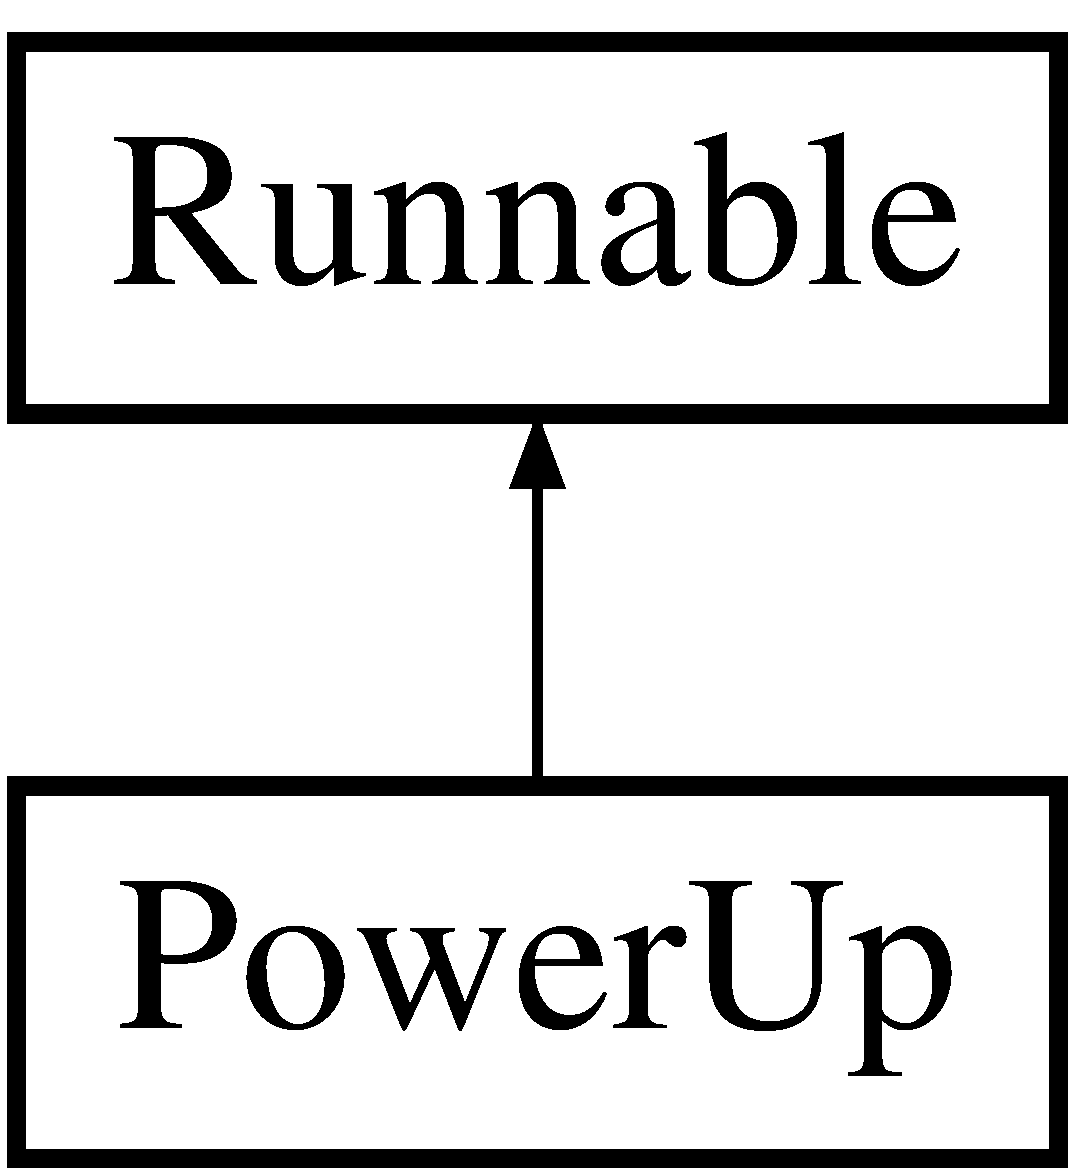
\includegraphics[height=2.000000cm]{class_power_up}
\end{center}
\end{figure}
\subsection*{Public Member Functions}
\begin{DoxyCompactItemize}
\item 
\hyperlink{class_power_up_a83f8659ad751f6b45f64afc55d035bbb}{Power\+Up} ()
\item 
\hyperlink{class_power_up_ac332a2e85c0f3e55388377a8f9ed7b3e}{Power\+Up} (int x\+Location, int y\+Location)
\item 
void \hyperlink{class_power_up_ab6f51e1081d0dbf3bacaa2835d4ccc11}{run} ()
\item 
void \hyperlink{class_power_up_a6fd36c59cebaad89b702cfee231ddf31}{destroy\+Power\+Up} ()
\end{DoxyCompactItemize}


\subsection{Constructor \& Destructor Documentation}
\hypertarget{class_power_up_a83f8659ad751f6b45f64afc55d035bbb}{}\index{Power\+Up@{Power\+Up}!Power\+Up@{Power\+Up}}
\index{Power\+Up@{Power\+Up}!Power\+Up@{Power\+Up}}
\subsubsection[{Power\+Up()}]{\setlength{\rightskip}{0pt plus 5cm}Power\+Up.\+Power\+Up (
\begin{DoxyParamCaption}
{}
\end{DoxyParamCaption}
)}\label{class_power_up_a83f8659ad751f6b45f64afc55d035bbb}
\hypertarget{class_power_up_ac332a2e85c0f3e55388377a8f9ed7b3e}{}\index{Power\+Up@{Power\+Up}!Power\+Up@{Power\+Up}}
\index{Power\+Up@{Power\+Up}!Power\+Up@{Power\+Up}}
\subsubsection[{Power\+Up(int x\+Location, int y\+Location)}]{\setlength{\rightskip}{0pt plus 5cm}Power\+Up.\+Power\+Up (
\begin{DoxyParamCaption}
\item[{int}]{x\+Location, }
\item[{int}]{y\+Location}
\end{DoxyParamCaption}
)}\label{class_power_up_ac332a2e85c0f3e55388377a8f9ed7b3e}


\subsection{Member Function Documentation}
\hypertarget{class_power_up_a6fd36c59cebaad89b702cfee231ddf31}{}\index{Power\+Up@{Power\+Up}!destroy\+Power\+Up@{destroy\+Power\+Up}}
\index{destroy\+Power\+Up@{destroy\+Power\+Up}!Power\+Up@{Power\+Up}}
\subsubsection[{destroy\+Power\+Up()}]{\setlength{\rightskip}{0pt plus 5cm}void Power\+Up.\+destroy\+Power\+Up (
\begin{DoxyParamCaption}
{}
\end{DoxyParamCaption}
)}\label{class_power_up_a6fd36c59cebaad89b702cfee231ddf31}
\hypertarget{class_power_up_ab6f51e1081d0dbf3bacaa2835d4ccc11}{}\index{Power\+Up@{Power\+Up}!run@{run}}
\index{run@{run}!Power\+Up@{Power\+Up}}
\subsubsection[{run()}]{\setlength{\rightskip}{0pt plus 5cm}void Power\+Up.\+run (
\begin{DoxyParamCaption}
{}
\end{DoxyParamCaption}
)}\label{class_power_up_ab6f51e1081d0dbf3bacaa2835d4ccc11}


The documentation for this class was generated from the following file\+:\begin{DoxyCompactItemize}
\item 
C\+:/\+Users/\+Ren-\/\+David/workspace/bomber\+Clone/src/\hyperlink{_power_up_8java}{Power\+Up.\+java}\end{DoxyCompactItemize}

\hypertarget{class_power_up_manager}{}\section{Power\+Up\+Manager Class Reference}
\label{class_power_up_manager}\index{Power\+Up\+Manager@{Power\+Up\+Manager}}
Inheritance diagram for Power\+Up\+Manager\+:\begin{figure}[H]
\begin{center}
\leavevmode
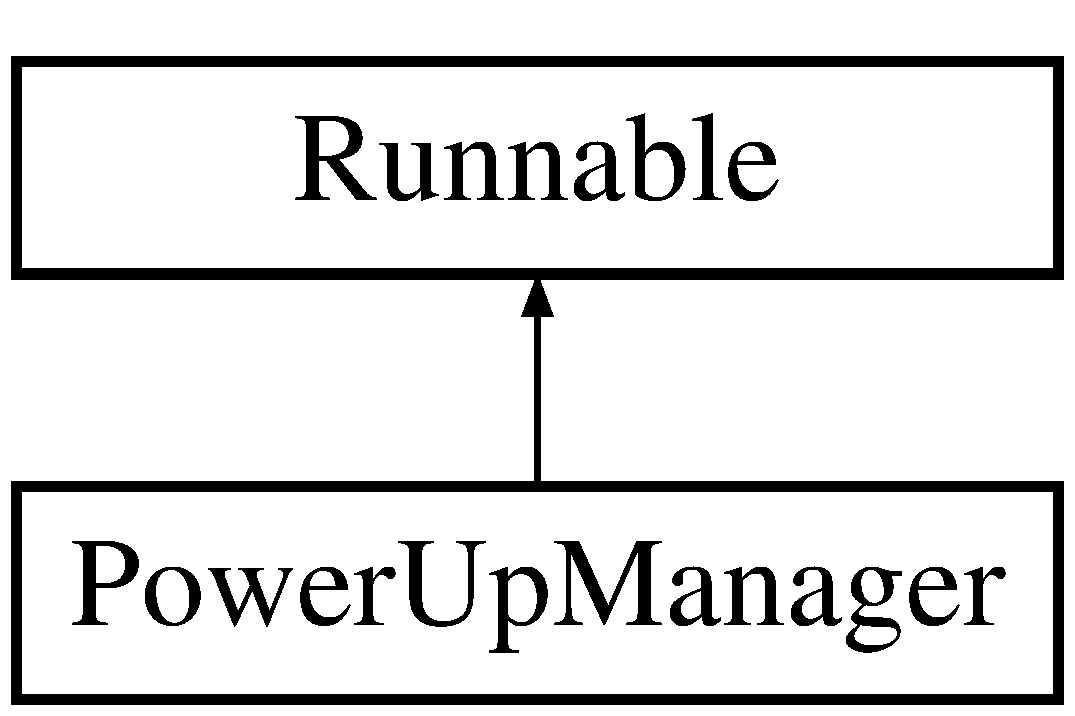
\includegraphics[height=2.000000cm]{class_power_up_manager}
\end{center}
\end{figure}
\subsection*{Public Member Functions}
\begin{DoxyCompactItemize}
\item 
\hyperlink{class_power_up_manager_a34087d5aaa60b4aaca89e97c06e5c1bf}{Power\+Up\+Manager} ()
\item 
void \hyperlink{class_power_up_manager_a04cf47b26d1f0b3ff7f93352a82a7d63}{start\+Power\+Ups} ()
\item 
void \hyperlink{class_power_up_manager_aa4b03f51b370e56120cec0bfc6869530}{run} ()
\end{DoxyCompactItemize}


\subsection{Constructor \& Destructor Documentation}
\hypertarget{class_power_up_manager_a34087d5aaa60b4aaca89e97c06e5c1bf}{}\index{Power\+Up\+Manager@{Power\+Up\+Manager}!Power\+Up\+Manager@{Power\+Up\+Manager}}
\index{Power\+Up\+Manager@{Power\+Up\+Manager}!Power\+Up\+Manager@{Power\+Up\+Manager}}
\subsubsection[{Power\+Up\+Manager()}]{\setlength{\rightskip}{0pt plus 5cm}Power\+Up\+Manager.\+Power\+Up\+Manager (
\begin{DoxyParamCaption}
{}
\end{DoxyParamCaption}
)}\label{class_power_up_manager_a34087d5aaa60b4aaca89e97c06e5c1bf}


\subsection{Member Function Documentation}
\hypertarget{class_power_up_manager_aa4b03f51b370e56120cec0bfc6869530}{}\index{Power\+Up\+Manager@{Power\+Up\+Manager}!run@{run}}
\index{run@{run}!Power\+Up\+Manager@{Power\+Up\+Manager}}
\subsubsection[{run()}]{\setlength{\rightskip}{0pt plus 5cm}void Power\+Up\+Manager.\+run (
\begin{DoxyParamCaption}
{}
\end{DoxyParamCaption}
)}\label{class_power_up_manager_aa4b03f51b370e56120cec0bfc6869530}
\hypertarget{class_power_up_manager_a04cf47b26d1f0b3ff7f93352a82a7d63}{}\index{Power\+Up\+Manager@{Power\+Up\+Manager}!start\+Power\+Ups@{start\+Power\+Ups}}
\index{start\+Power\+Ups@{start\+Power\+Ups}!Power\+Up\+Manager@{Power\+Up\+Manager}}
\subsubsection[{start\+Power\+Ups()}]{\setlength{\rightskip}{0pt plus 5cm}void Power\+Up\+Manager.\+start\+Power\+Ups (
\begin{DoxyParamCaption}
{}
\end{DoxyParamCaption}
)}\label{class_power_up_manager_a04cf47b26d1f0b3ff7f93352a82a7d63}


The documentation for this class was generated from the following file\+:\begin{DoxyCompactItemize}
\item 
C\+:/\+Users/\+Ren-\/\+David/workspace/bomber\+Clone/src/\hyperlink{_power_up_manager_8java}{Power\+Up\+Manager.\+java}\end{DoxyCompactItemize}

\chapter{File Documentation}
\hypertarget{_bomb_8java}{}\section{C\+:/\+Users/\+Ren-\/\+David/workspace/bomber\+Clone/src/\+Bomb.java File Reference}
\label{_bomb_8java}\index{C\+:/\+Users/\+Ren-\/\+David/workspace/bomber\+Clone/src/\+Bomb.\+java@{C\+:/\+Users/\+Ren-\/\+David/workspace/bomber\+Clone/src/\+Bomb.\+java}}
\subsection*{Classes}
\begin{DoxyCompactItemize}
\item 
class \hyperlink{class_bomb}{Bomb}
\end{DoxyCompactItemize}

\hypertarget{_bomberman_8java}{}\section{C\+:/\+Users/\+Ren-\/\+David/workspace/bomber\+Clone/src/\+Bomberman.java File Reference}
\label{_bomberman_8java}\index{C\+:/\+Users/\+Ren-\/\+David/workspace/bomber\+Clone/src/\+Bomberman.\+java@{C\+:/\+Users/\+Ren-\/\+David/workspace/bomber\+Clone/src/\+Bomberman.\+java}}
\subsection*{Classes}
\begin{DoxyCompactItemize}
\item 
class \hyperlink{class_bomberman}{Bomberman}
\end{DoxyCompactItemize}

\hypertarget{_menu_8java}{}\section{C\+:/\+Users/\+Ren-\/\+David/workspace/bomber\+Clone/src/\+Menu.java File Reference}
\label{_menu_8java}\index{C\+:/\+Users/\+Ren-\/\+David/workspace/bomber\+Clone/src/\+Menu.\+java@{C\+:/\+Users/\+Ren-\/\+David/workspace/bomber\+Clone/src/\+Menu.\+java}}
\subsection*{Classes}
\begin{DoxyCompactItemize}
\item 
class \hyperlink{class_menu}{Menu}
\end{DoxyCompactItemize}

\hypertarget{_options_8java}{}\section{C\+:/\+Users/\+Ren-\/\+David/workspace/bomber\+Clone/src/\+Options.java File Reference}
\label{_options_8java}\index{C\+:/\+Users/\+Ren-\/\+David/workspace/bomber\+Clone/src/\+Options.\+java@{C\+:/\+Users/\+Ren-\/\+David/workspace/bomber\+Clone/src/\+Options.\+java}}
\subsection*{Classes}
\begin{DoxyCompactItemize}
\item 
class \hyperlink{class_options}{Options}
\end{DoxyCompactItemize}

\hypertarget{_player_8java}{}\section{C\+:/\+Users/\+Ren-\/\+David/workspace/bomber\+Clone/src/\+Player.java File Reference}
\label{_player_8java}\index{C\+:/\+Users/\+Ren-\/\+David/workspace/bomber\+Clone/src/\+Player.\+java@{C\+:/\+Users/\+Ren-\/\+David/workspace/bomber\+Clone/src/\+Player.\+java}}
\subsection*{Classes}
\begin{DoxyCompactItemize}
\item 
class \hyperlink{class_player}{Player}
\end{DoxyCompactItemize}

\hypertarget{_power_up_8java}{}\section{C\+:/\+Users/\+Ren-\/\+David/workspace/bomber\+Clone/src/\+Power\+Up.java File Reference}
\label{_power_up_8java}\index{C\+:/\+Users/\+Ren-\/\+David/workspace/bomber\+Clone/src/\+Power\+Up.\+java@{C\+:/\+Users/\+Ren-\/\+David/workspace/bomber\+Clone/src/\+Power\+Up.\+java}}
\subsection*{Classes}
\begin{DoxyCompactItemize}
\item 
class \hyperlink{class_power_up}{Power\+Up}
\end{DoxyCompactItemize}

\hypertarget{_power_up_manager_8java}{}\section{C\+:/\+Users/\+Ren-\/\+David/workspace/bomber\+Clone/src/\+Power\+Up\+Manager.java File Reference}
\label{_power_up_manager_8java}\index{C\+:/\+Users/\+Ren-\/\+David/workspace/bomber\+Clone/src/\+Power\+Up\+Manager.\+java@{C\+:/\+Users/\+Ren-\/\+David/workspace/bomber\+Clone/src/\+Power\+Up\+Manager.\+java}}
\subsection*{Classes}
\begin{DoxyCompactItemize}
\item 
class \hyperlink{class_power_up_manager}{Power\+Up\+Manager}
\end{DoxyCompactItemize}

%--- End generated contents ---

% Index
\backmatter
\newpage
\phantomsection
\clearemptydoublepage
\addcontentsline{toc}{chapter}{Index}
\printindex

\end{document}
